% D.12 一线三等角：等边△ABC，D∈BC、E∈AC，∠ADE=60°
\documentclass[tikz,border=4pt]{standalone}
\usepackage{ctex}
\usepackage{amsmath}
\usetikzlibrary{calc}
\begin{document}
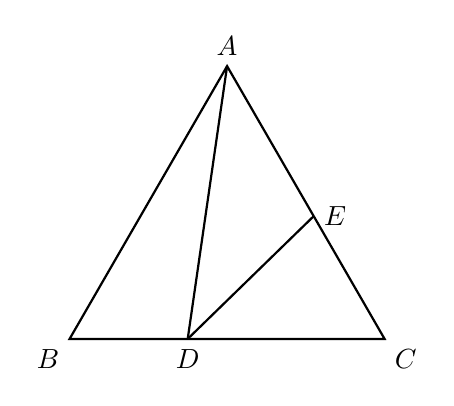
\begin{tikzpicture}[scale=1.0, thick]
  \coordinate (B) at (0, 0);
  \coordinate (C) at (4, 0);
  \coordinate (A) at (2, {2*sqrt(3)});
  \coordinate (D) at (1.5, 0);
  % E 在 AC 上，使 ∠ADE = 60°
  % 直接给一个目测合理位置
  \coordinate (E) at ($(A)!0.55!(C)$);

  \draw (A) -- (B) -- (C) -- cycle;
  \draw (A) -- (D);
  \draw (D) -- (E);

  \node[above]       at (A) {$A$};
  \node[below left]  at (B) {$B$};
  \node[below right] at (C) {$C$};
  \node[below]       at (D) {$D$};
  \node[right]       at (E) {$E$};
\end{tikzpicture}
\end{document}
